\documentclass[crop=true, border=10pt]{standalone}

\usepackage{amsmath}
 
\usepackage{graphicx}
\usepackage{xcolor}

\usepackage{tikz}
\usetikzlibrary{arrows.meta}

\usepackage{tikz-3dplot}

\usepackage{pgfplots}
\usepgfplotslibrary{fillbetween}

\definecolor{plum}{rgb}{0.36078, 0.20784, 0.4}
\definecolor{chameleon}{rgb}{0.30588, 0.60392, 0.023529}
\definecolor{cornflower}{rgb}{0.12549, 0.29020, 0.52941}
\definecolor{scarlet}{rgb}{0.8, 0, 0}
\definecolor{brick}{rgb}{0.64314, 0, 0}
\definecolor{sunrise}{rgb}{0.80784, 0.36078, 0}
\definecolor{lightblue}{rgb}{0.15,0.35,0.75}

\newcommand\nts{\negthickspace} 

\pgfplotsset{width=9cm,compat=1.15}

\begin{document}


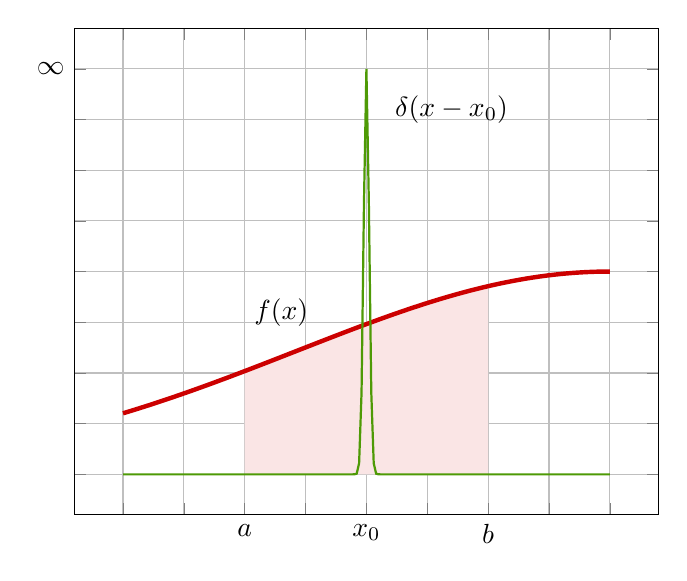
\begin{tikzpicture}
\begin{axis}[%xlabel=$x$,
	ylabel=,grid=both,xtick=\empty,ytick=\empty, minor tick num=2,
	extra x ticks={-1,-.5,0,.5,1,1.5,2,2.5,3},
    extra x tick style={grid=major},
    extra x tick labels={,,$a$,,$x_{0}$,,$b$,,},
	extra y ticks={0,.125,.25,.375,.5,.625,.75,.875,1},
    extra y tick style={grid=major,},
    extra y tick labels={,,,,,,,,$\infty$},
]
    \addplot [
		name path = A,
        scarlet, ultra thick,
        domain=-1:3,
        samples=201,
    ]
        {.5*exp(-.075*(x-3)^2)};
%
	 \path [name path=B]
        (0,0) -- (2,0);
%
 	\addplot [scarlet!10] fill between [
	        of=A and B,
	        soft clip={
	            (0,0) rectangle (2,4)
	},
	];
%
    % Dirac Delta
    \addplot [
        chameleon, thick,
        domain=-1:3,
        samples=201,
    ]
        {exp(-1000*(x-1)^2)};
%
	\node [] at (1.7,.9) {$\delta(x-x_{0})$};
	\node [] at (.3,.4) {$f(x)$};
\end{axis}
\end{tikzpicture}
%
\hskip1em
%
\begin{tikzpicture}
	% Set the first node so bottom corners of both pictures are at the same height.
	\node [] at (0,0) {};
	\node [] at (0,3.5) {$\displaystyle \int_{a}^{b} \nts dx\,f(x)\,\delta(x-x_{0}) = f(x_{0})$};
\end{tikzpicture}



\end{document}